\colorlet{chaptergrey}{gray}
\chapter[The relationship between black activity and simulated IFU kinematics in IllustrisTNG]{Misalignment and black hole activity}
\label{ch:halo_assembly}
\vspace{-5.25in}
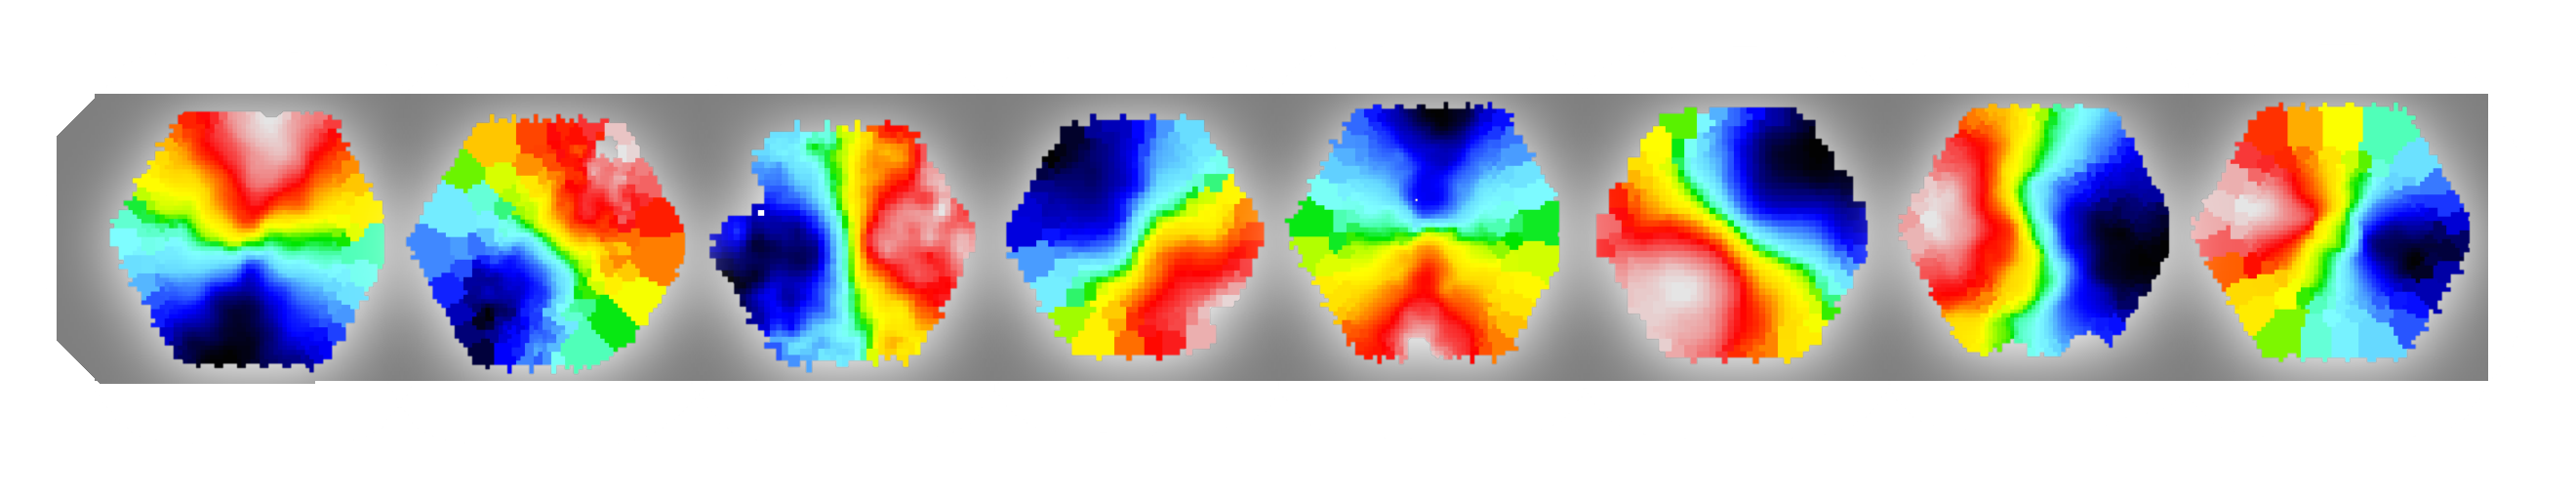
\includegraphics[height=1.39in]{thesis/latex/misalignment_intro/kin_mis_chapter_heading_grey.pdf}
\vspace{3in}

\epigraph{This chapter is based Duckworth, Starkenburg, Genel, Davis, Habouzit, Kraljic and Tojeiro (submitted). Here we investigate the temporal relationship between kinematically misaligned galaxies and black hole activity in IllustrisTNG.}

\section{Introduction}
Recent cosmological scale hydro-dynamical simulations have provided a clear insight into the relationship between the angular momentum of baryons and dark matter through cosmic time. A necessary component of realistic simulations is efficient feedback from both supermassive black holes (BH) and stars, required to, amongst other things, reproduce late type disks and solve the problem of catastrophic angular momentum loss \citep[e.g.][]{zavala2008, scannapieco2009}. Active galactic nuclei (AGN) and supernova explosions can also lead to dramatic redistribution of gas which regulate the angular momentum content of galaxies \citep[e.g.][]{genel2015, DeFelippis2017}.

`Quasar' (radiative) mode feedback releases huge amounts of energy through radiation from the accretion disk leading to high luminosity AGN and dramatic gas outflows \citep[e.g.][]{cattaneo2009, rubin2014, cheung2016}. Alternatively `radio' (kinetic) mode \red{a term} for lower luminosity AGN that host lower black hole accretion rates. In this instance energy is deposited into the surrounding gas via jets which drive outflows, heat the gas and suppress star formation \citep[][]{binney1995, ciotti2001, heckman2014}.

The relationship between AGN and kinematics has been the focus of several recent studies using data from Integral Field Spectroscopy. In particular, a potential new class of galaxy termed `red geyser' has been identified which host AGN and exhibit high velocity outflows in the spatial distribution of ionized gas \citep[][]{cheung2016, roy2018}. These outflows are often linked to a distinctive offset in rotation direction between the stars and gas. Detection of ongoing outflows is, however, rare ($\sim5-10$\% of the quiescent population). \citet{penny2018} demonstrate the importance of AGN feedback in low mass quiescent galaxies ($\mathrm{M_{stel} < 5 \times 10^{9}M_{\odot}}$). While the majority demonstrate no ionized gas present, quiescent galaxies (i.e. with reduced or null SFR) with an AGN show a clear decoupling in the rotation of stars and gas. However, the relationship of gas kinematics to BH feedback is not clear for all galaxies \citep[see also:][]{koudmani2019}. In particular, \citet{ilha2019} find that the typical decoupling between stars and gas for AGN defined galaxies are consistent with an inactive control sample. 

As introduced in \red{section X}, the decoupled rotation of stars and gas can be a natural result of external processes \cite[e.g.][]{davis2011, barrera2015, vdvoort2015, jin2016, bryant2019, duckworth2019_halo, li_decoupling2019}. Regardless of internal or external origin, kinematic misalignment in observations and simulations is linked with both a lower gas mass fraction and angular momentum as demonstrated in \red{section Y} \citep[see also;][]{starkenburg+19, khim2019}. In particular, \citet{starkenburg+19} highlight the importance of feedback leading to gas loss, enabling new or re-accretion as a mechanism for future misalignment in low mass galaxies. The question arises if misalignment is caused in the first instance by mergers or cosmic gas accretion (and hence making BH accretion easier) or if they are a result of AGN feedback leading to gas loss allowing for accretion of misaligned gas. The timescales of luminous AGN are typically much shorter than kinematic misalignment, making correlation at $z=0$ alone difficult. 

In this chapter, we study the temporal relationship between BH feedback, BH luminosity and kinematic misalignment in the cosmological scale hydrodynamical simulation of IllustrisTNG100 (hereafter referred to as TNG100). We use our sample of galaxies with mock MaNGA observations introduced in \red{section Z} to emulate what we may expect to see in IFS observations. In Section \ref{sec:methods_BH} we briefly introduce the specific methods associated with this work, before introducing results in Section \ref{sec:results_BH}. Finally we summarise the chapter in Section \ref{sec:summary_BH}.

\section{Methods} \label{sec:methods_BH}
As introduced in \S\ref{sec:sim_data_TNG}, we make use of data from the IllustrisTNG100 simulation. For studies of black hole properties, of particular relevance is the prescription of \citet{weinberger17} for BH feedback, which is modelled by two modes (quasar mode: high accretion, kinetic mode: low accretion). The transition threshold in terms of the Eddington ratio is $\mathrm{f_{Edd}= \min ( 2x10^{-3}(M_{BH}/10^8 M_{\odot})^2 , 0.1)}$ so that BHs typically transition from quasar to kinetic mode around $\mathrm{M_{BH} = 10^{8}M_{\odot}}$. In the following, we separate our TNG100 galaxies by stellar mass at $\mathrm{M_{stel} = 10^{10.2}M_{\odot}}$ (nominally referred to low and high mass galaxies henceforth) which corresponds to this transition \citep[i.e. $\mathrm{M_{BH} \approx 10^{8}M_{\odot}}$, see Fig 1 in][]{li2019}. We do not explicitly follow the individual modes of accretion and feedback for each galaxy, which can alternate through its evolutionary history. Despite this, the transition threshold in TNG determines that we almost exclusively isolate the role of radiative feedback for our low mass sample. Our high mass sample, however, has been subject to both quasar and kinetic feedback over the last 8 Gyrs. To emulate what we may expect to see in IFS observations, we make use of our mock MaNGA sample as introduced in \S\ref{sec:mock_obs}.

\red{move to first introduction of following properties back in time?} The prior time evolution of BH and gas properties for each galaxy is followed by considering the main progenitor branch (most massive defined by stellar mass) in the sublink merger trees \citep{rgomez2015}. We compute BH bolometric luminosities as:
\begin{equation}
\mathrm{L_{bol, AGN}} = \frac{\varepsilon_r}{1 - \varepsilon_r} \dot{\mathrm{M}}_{\mathrm{BH}} \mathrm{c^2}
\end{equation}
where $\varepsilon_r=0.1$ is the radiative efficiency \citep[see discussion in][]{habouzit2019}, c the light speed, and $\dot{\mathrm{M}}_{\mathrm{BH}}$ the accretion rate onto the BH. Gas properties are defined within two effective radii ($\mathrm{R_{e}}$, radius containing half of the stellar mass within the galaxy), unless stated otherwise.

\section{Results} \label{sec:results_BH}
Each panel of Figure \ref{fig:overall_pop} shows the time evolution average of a property for all galaxies split by stellar mass at $\mathrm{M_{stel} = 10^{10.2}M_{\odot}}$, as explained in \S\ref{sec:methods}. Splitting directly on BH mass at $\mathrm{M_{BH} = 10^{8}M_{\odot}}$ or enforcing stricter stellar mass cuts does not change any of our findings. We divide our sample by $\Delta$PA at $z=0$. For each sub-population, we find that the stellar mass distributions are consistent at $z=0$ for aligned and misaligned galaxies. We also split on specific star formation rate using the distance from the star-forming sequence (SFS) as defined in \citet{pillepich2019}. We select star forming ($\Delta \mathrm{log_{10}(SFR) > -0.5}$) and quenched galaxies ($\Delta \mathrm{log_{10}(SFR) \leq -1.0}$) at $z=0$. For clarity, the correlations with each misaligned sub-population in Figure \ref{fig:overall_pop} are summarized by Table \ref{tab:truth}. Additional time evolution properties can be found in the Supplementary material, and are also summarized in Table \ref{tab:truth}.

\begin{figure}
	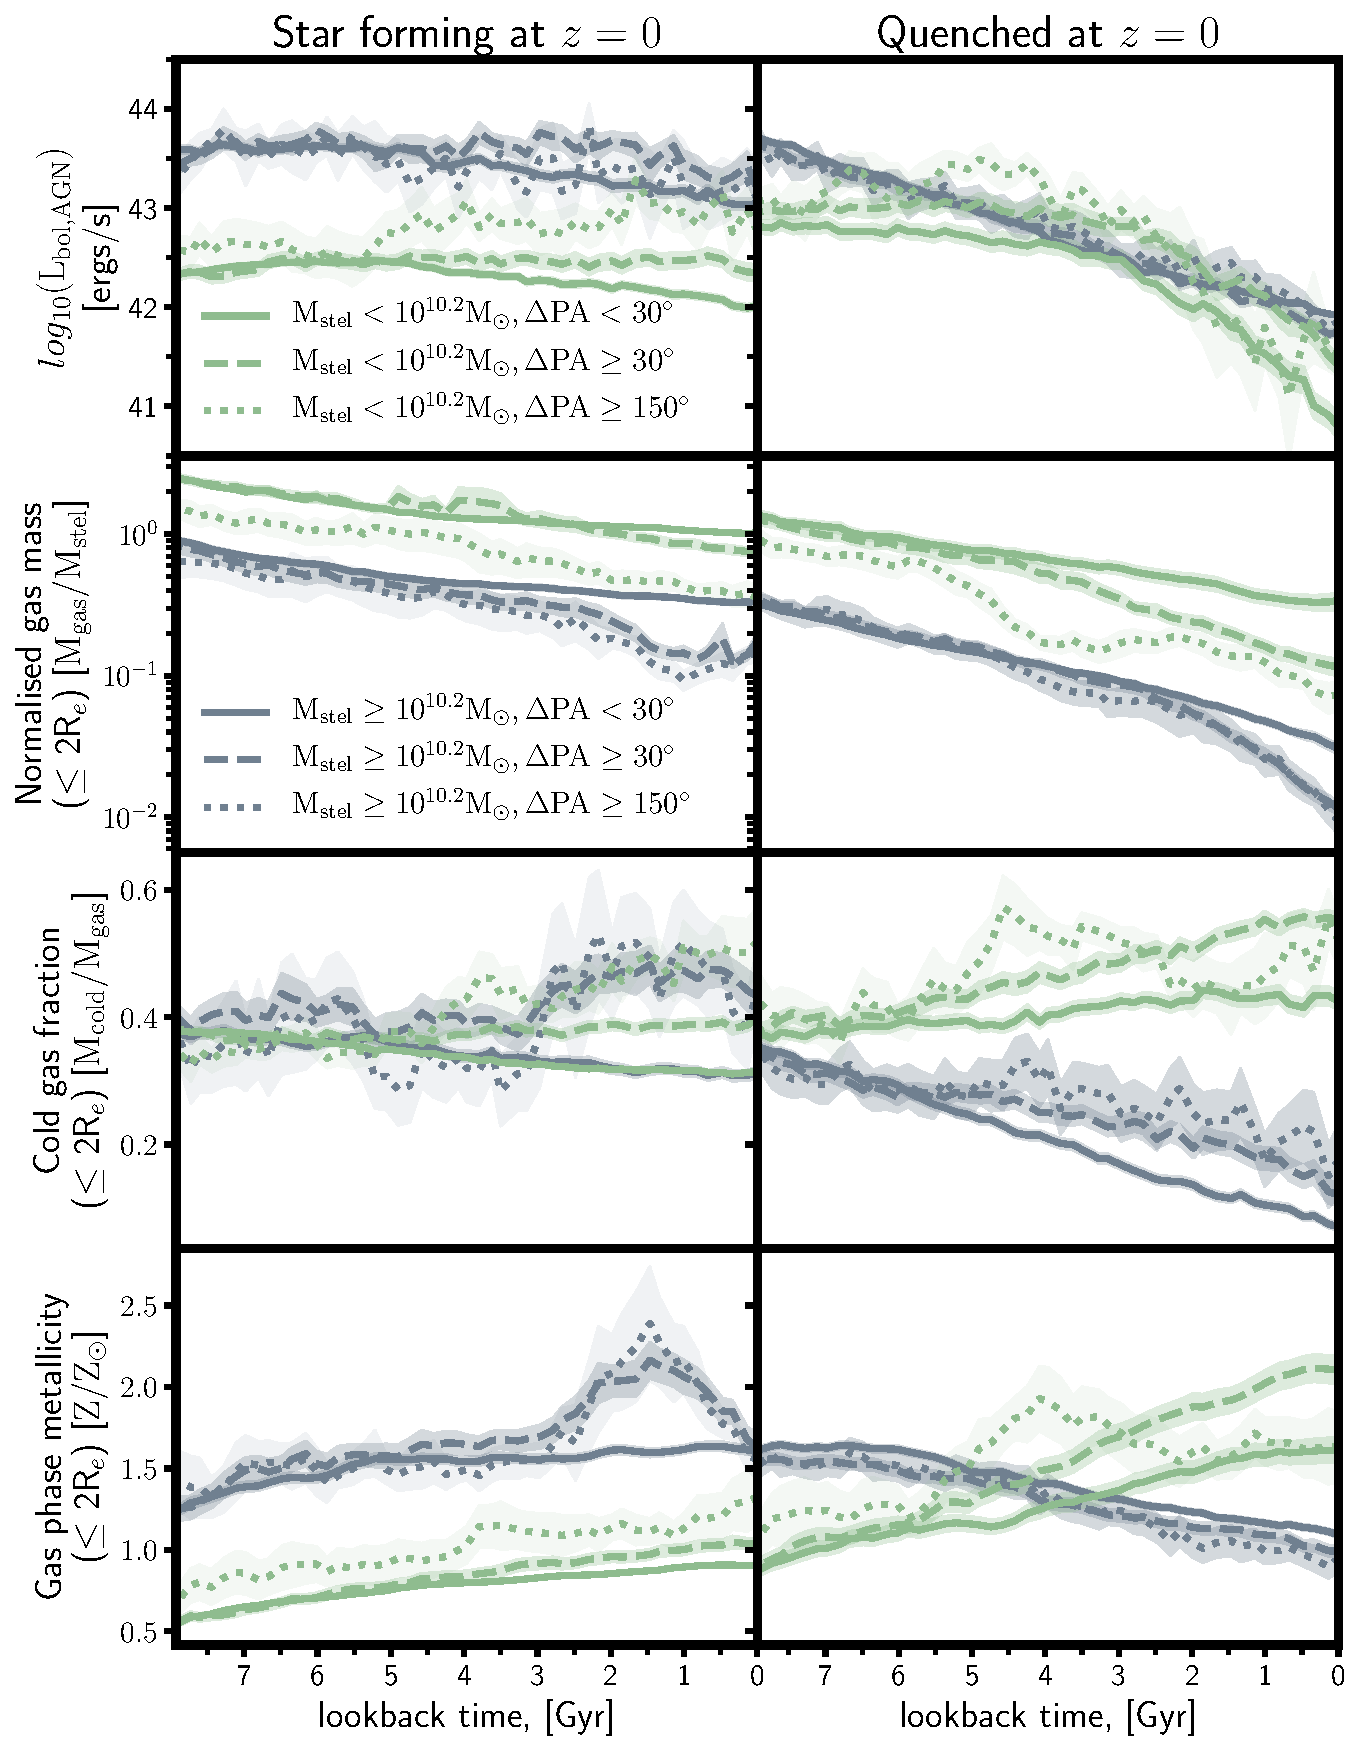
\includegraphics[width=\linewidth]{misalignment_BH/time_evo_letter_without_BH_props.pdf}
    \caption{Time evolution of (rows top to bottom) black hole luminosity ($\mathrm{log_{10}(L_{bol, AGN})}$), normalised gas mass ($\mathrm{M_{gas}/M_{stel}}$), cold and star forming gas fraction ($\mathrm{M_{cold}/M_{stel}}$), and, gas phase metallicity for star forming (left) and quenched galaxies (right) identified at $z=0$. Galaxies are divided into low mass (green; $\mathrm{M_{stel} < 10^{10.2}M_{\odot}}$) and high mass (grey; $\mathrm{M_{stel} > 10^{10.2}M_{\odot}}$) populations. Both are subdivided by misalignment ($\Delta$PA $< 30^{\circ}$: solid, $\geq 30^{\circ}$: dashed, and  $\geq 150^{\circ}$: dotted). Each line shows the mean for the population with the shaded region corresponding to the standard error.
    }
    \label{fig:overall_pop}
\end{figure}

\begin{figure}
	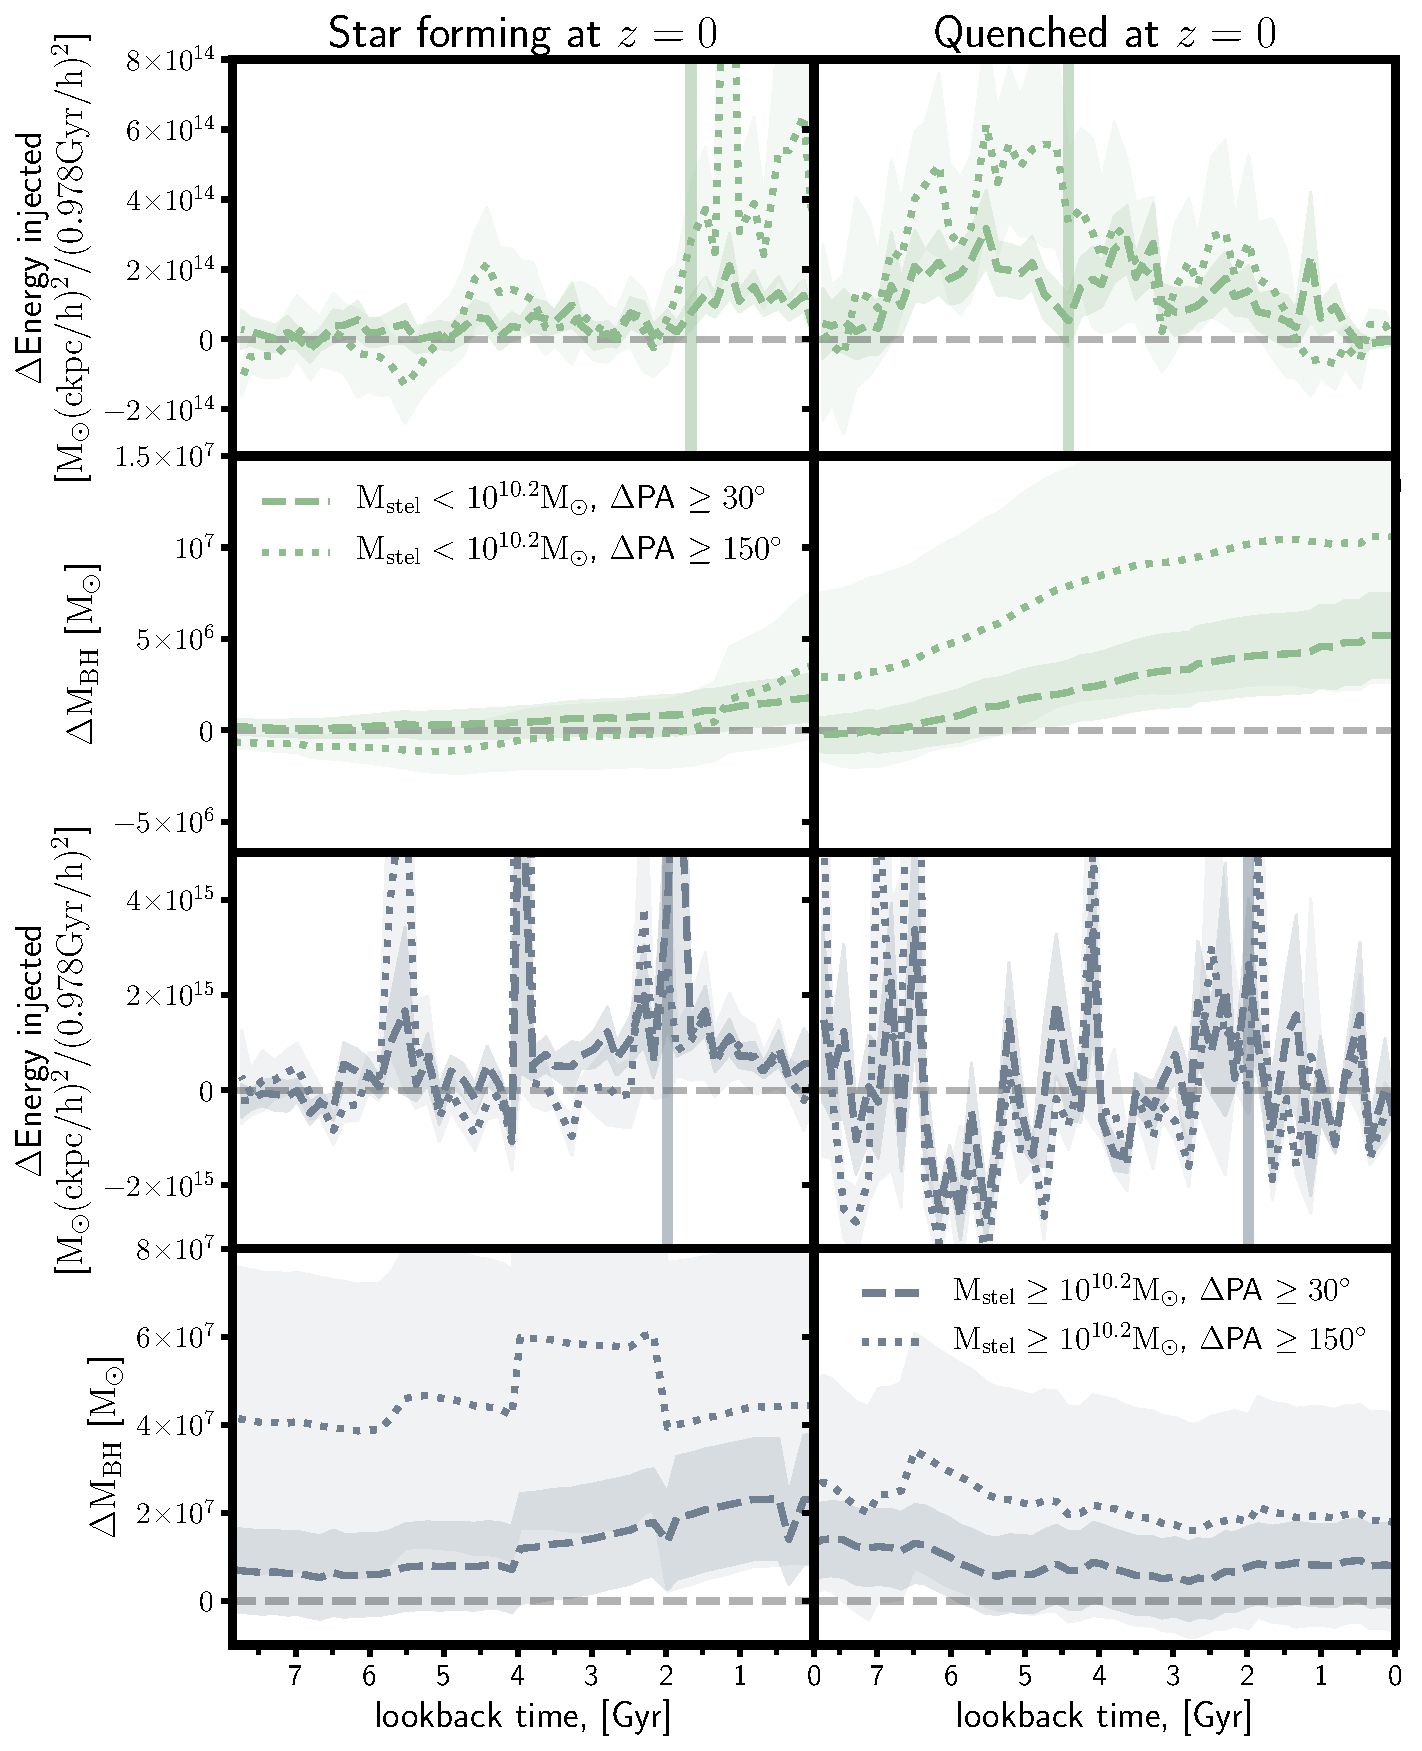
\includegraphics[width=\linewidth]{misalignment_BH/BH_props_only.pdf}
    \caption{\red{Time evolution of black hole feedback energy injection and black hole mass for star forming (left) and quenched galaxies (right). Each row shows the residuals ($\Delta$Energy injected$\mathrm{ = E_{Misaligned/Counter-rotating} - E_{Aligned}}$) or $\Delta \mathrm{M_{BH}}$ where galaxies with $\Delta$PA $\geq 30^{\circ}$ (dashed) and $\Delta$PA $\geq 150^{\circ}$ (dotted) are defined relative to $\Delta$PA$ < 30^{\circ}$. The vertical line in the energy injection panels represents the time at which 50\% of the energy over the last 8 Gyrs has been injected. The top (bottom) two rows show the trends for low (high) mass galaxies.}}
    \label{fig:BH_props}
\end{figure}

\begin{adjustbox}{angle=90}
\begin{tabular}{llllllll}
\hline
&  $\mathrm{L_{bol,AGN}}$ & $\mathrm{M_{gas} / M_{stel} (< 2R_e)}$ & $\mathrm{M_{cold} / M_{gas}}$ & $\mathrm{Z / Z_{\odot}}$ & $\mathrm{M_{gas}/M_{stel} (total)}$ & $\mathrm{M_{cold}/M_{stel}}$ & $\mathrm{j_{star}}$ \\
\hline
Low mass star forming & ++ & $--$ & ++ & + & $--$ & 0/$-$C & $--$ \\
High mass star forming & + & $-$/bump & ++/bump & ++/bump & $--$ & -/bump & $--$ \\
Low mass quenched & +/bumpC & $--$/bumpC & ++/bumpC & ++/bumpC & $--$ & $--$ & $--$ \\
High mass quenched & 0 & $-$ & ++ & 0$-$ & 0 & 0+ & $--$ \\
\end{tabular}
\caption{Truth table summarising the correlations found in Figure \ref{fig:overall_pop} between BH luminosity, normalised gas mass ($\mathrm{< 2R_e}$), cold gas fraction and gas phase metallicity (first four columns) with misalignment identified at $z=0$. The latter three columns additionally show the correlations found in the Supplementary material between total normalised gas mass (in subhalo), normalised cold gas mass and specific stellar angular momentum with misalignment. Correlations are shown individually for misaligned galaxies separated by both stellar mass and SFR at $z=0$. ++, + ($--$, $-$) refer to strong and mild positive (negative) correlations, 0 to no correlation and bump indicates a feature in the curve. A C is appended if the correlation/feature is only applicable to counter-rotating galaxies.}
\label{tab:truth}
\end{adjustbox}

\section{Summary} \label{sec:summary_BH}
